\section{Brief introduction to the Lojban grammar}

Lojban sentences are constructed in a way that expresses a logical predicate, with a fixed set of arguments. For a small
refresher course in predicate logic see Annex A. The recurring ``first approach to the language'' example used in most Lojban
literature, from the language standard to research papers is the sentence ``John is the father of Sam''. In this sentence, there
is a clear predicate (``is-the-father-of'') and two arguments (``John'' and ``Sam'').

\begin{figure}[H]
\centering
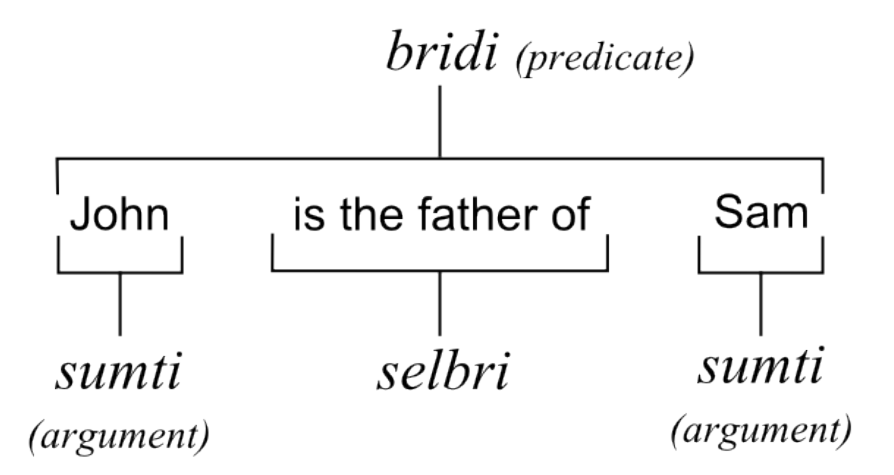
\includegraphics[scale=0.20]{images/lojban_grammar.png}
\caption{Basic structure of a Lojban sentence (Source: \cite{cowan1997complete})}
\end{figure}

This figure presents the three most important base elements of a sentence in Lojban:

\begin{itemize}
    \item \textbf{bridi}: the predicate expression;
    \item \textbf{selbri}: the word(s) acting as the predicate;
    \item \textbf{sumti}: positional argument passed to the predicate.
\end{itemize}

Selbri are strictly defined by representations which position the sumti around a key word. For example, the selbri to describe the fatherhood relationship is ``patfu'':

$$\text{patfu}: x_1 \: \text{is a father of} \: x_2$$

Thus, the above sentence is expressed in Lojban as: \textbf{la .djon. patfu la .sam.} \newline

If no modifiers are used, the position of the sumti is rigid and allows to release the sentence from any ambiguity. We always know who is the father and who is the child.
Of course, in this example, the English counterpart doesn't really make sense (the sentence ``Sam is `fathered' by John'' makes absolutely no sense), but for a non-native speaker
the order of words in other pairs of sentences might add ambiguity. For example, a non-native might get confused about the difference between the sentences
``My dog bites the man'' (\textbf{``le mi gerku cu batci le nanmu''} in Lojban) and ``The man is being bitten by my dog'', as this inverted construct might not exist in their language.
Lojban solves this issue by having a specific keyword, indicating that two or more sumti (positional arguments) are going to be swapped. This allows speakers, even those not
familiar with this grammatical construct, to understand the difference between two very different sentence constructions: e.g. ``The man is being bitten by my dog''
and ``The man is biting my dog''.\newline

Of course, this framework of predicate expressions is simply the base feature of the language, but many others allow it to cover the other missing aspects that most natural
languages feature: tenses, relative clauses, abstractions, emotional indicators, and many others. These will be explored in a further chapter of the thesis. \newline